\begin{figure}[H]
\centering
\resizebox{\textwidth}{!}{%
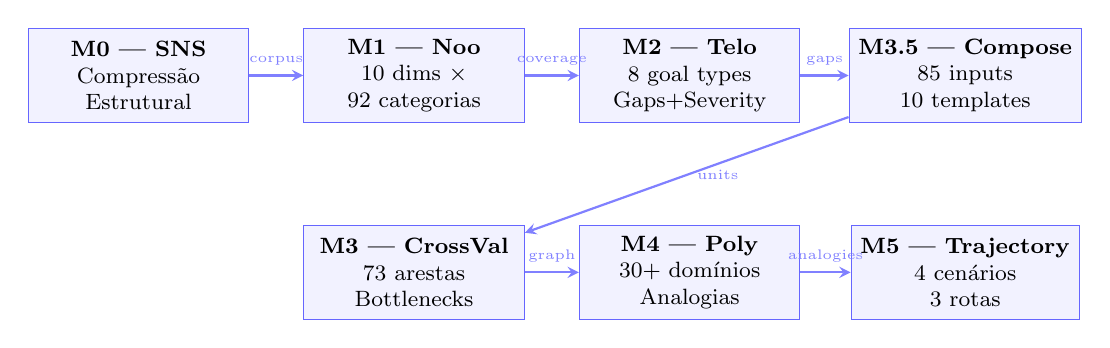
\begin{tikzpicture}[
    box/.style={rectangle, draw=blue!60, fill=blue!5, minimum width=2.8cm, minimum height=1.2cm, align=center, font=\footnotesize},
    arrow/.style={->, >=stealth, thick, blue!50},
]
\node[box] (M0) at (0,0) {\textbf{M0 — SNS}\\Compressão\\Estrutural};
\node[box] (M1) at (3.5,0) {\textbf{M1 — Noo}\\10 dims $\times$\\92 categorias};
\node[box] (M2) at (7,0) {\textbf{M2 — Telo}\\8 goal types\\Gaps+Severity};
\node[box] (M35) at (10.5,0) {\textbf{M3.5 — Compose}\\85 inputs\\10 templates};
\node[box] (M3) at (3.5,-2.5) {\textbf{M3 — CrossVal}\\73 arestas\\Bottlenecks};
\node[box] (M4) at (7,-2.5) {\textbf{M4 — Poly}\\30+ domínios\\Analogias};
\node[box] (M5) at (10.5,-2.5) {\textbf{M5 — Trajectory}\\4 cenários\\3 rotas};

\draw[arrow] (M0) -- (M1) node[midway,above,font=\tiny] {corpus};
\draw[arrow] (M1) -- (M2) node[midway,above,font=\tiny] {coverage};
\draw[arrow] (M2) -- (M35) node[midway,above,font=\tiny] {gaps};
\draw[arrow] (M35) -- (M3) node[midway,right,font=\tiny] {units};
\draw[arrow] (M3) -- (M4) node[midway,above,font=\tiny] {graph};
\draw[arrow] (M4) -- (M5) node[midway,above,font=\tiny] {analogies};
\end{tikzpicture}%
}
\caption{Pipeline de Scanners — Fluxo M0 $\rightarrow$ M5. O corpus passa por compressão estrutural (M0), diagnóstico epistemológico (M1), inferência teleológica (M2), decomposição em insumos (M3.5), validação cruzada (M3), convergência polimática (M4) e mapeamento de trajetórias (M5).}
\label{fig:scanner_pipeline}
\end{figure}
